% !TeX root = ../main.tex
% !TEX root = ../main.tex
% -*- root: ../main.tex -*-
% -*- program: pdflatex -*-
\chapter{刻度公式的适用性研究}
前面的三章都是以~MRPC~的模块编号为~55~,读数条的编号为~7~这一条读数条为例进行研究的。在之前的第二章介绍~BESIII~的~TOF-MRPC~的结构时,讲到现在的端盖~MRPC~有东西两部分组成,每部分~36~个模块。每个模块有~12~个读数条。共计~864~个读数条。显然,刻度公式需要对于这~864~个读数条都是适用的。这一章就是探讨刻度公式的适用性的问题。
\section{刻度常数及刻度后的时间分辨}
在第4章和第5章的研究中,对于击中位置的修正采用多项式修正;对于过阈时间的修正,进行了击中公式的比较。其中公式${p_{0}+p_{1}/\sqrt{q}+p_{2}/q}$是拟合比较的一个公式。基于此:这里选用公式如下:

单端:$p_{0}+p_{1}/\sqrt{q}+p_{2}/q+p_{3}*zrhit+p_{4}*zrhit^{2}+p_{5}*zrhit^{3}+p_{6}*zrhit^{4}$

双端:$p_{0}+p_{1}/\sqrt{q}+p_{2}/q+p_{3}*t_{sub}+p_{4}*t_{sub}^{2}+p_{5}*t_{sub}^{3}+p_{6}*t_{sub}^{4}$

其中对于单端:~q~表示的是过阈时间(TOT),~zrhit~表示的是击中位置;对于双端:~q~表示的是双端的过阈时间的平均值,$t_{sub}$表示的是测量的初始时间差的一半,即$t_{sub}$=($t_{left}$-$t_{right}$)/2,和~zrhit~量存在线性关系,可以用来修正击中位置。

%以此为刻度公式,选择2016年5月24日到5月30日的Bhabha事例为刻度样本,在~root~下,配置好刻度重建环境,写好刻度脚本,然后提交到~BESIII~集群上,完成刻度工作。

以此为刻度公式,选择~2016~年~5~月~24~日到~5~月~30~日的~Bhabha~事例为刻度样本,完成刻度工作。

\begin{figure}[!h]
\centering
\includegraphics[width=0.9\textwidth]{chap5/calibration-par.png}
\caption{刻度后截取的两个模块共~24~条读数条的刻度常数}
\label{fig:calibration-par}
\end{figure}
图~\ref{fig:calibration-par}~给出了单端刻度后的部分读数条的刻度常数。其中第一列表示的是一个行号,对应不同的读数条的编号。第二列表示的是刻度项的常数项,主要在~8-9~ns之间,之后的两项表示的是和过阈时间相关的刻度常数。最后的四项是和击中位置相关的刻度常数,其中的第一项基本在~0.055~ns/cm左右,基本和信号在读数条内传播的有效速度一致。

图~\ref{fig:calib-res-160524-30}~给出了这一周的数据刻度得到的单端和双端的整体的时间分辨。其中单端的为~67~ps,双端的为~56.6~ps。
\begin{figure}[!h]
\centering
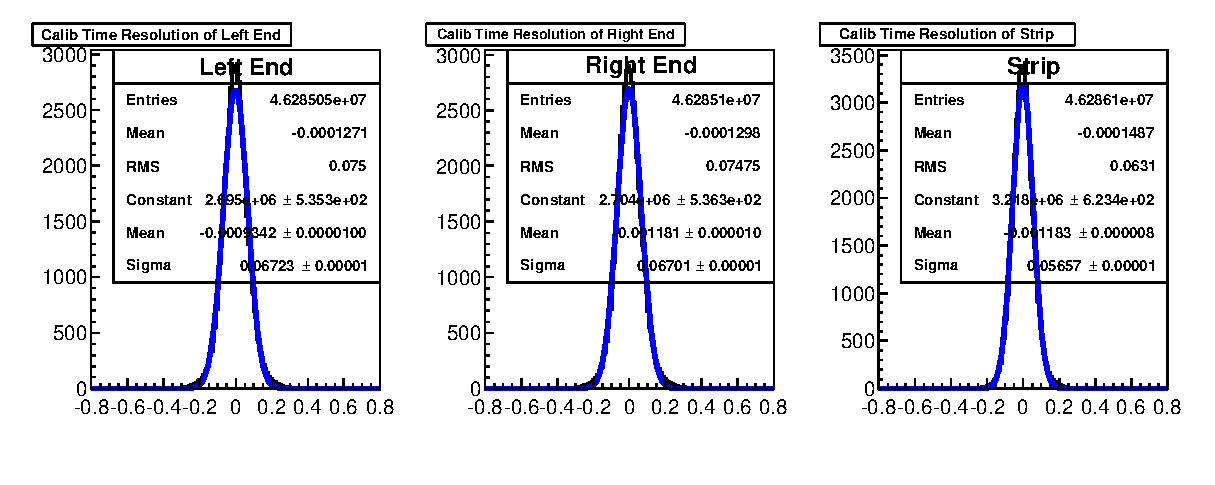
\includegraphics[width=0.9\textwidth]{chap5/calib-res-160524-30.eps}
\caption{最终整体的时间分辨}
\label{fig:calib-res-160524-30}
\end{figure}

图~\ref{fig:after-Calibration}~给出了刻度修正后时间对击中位置和过阈时间的分布。其中上面三幅图表示时间和击中位置的分布,分别为两个单端和一个双端;下面三幅图表示时间对过阈时间的分布,分别对应两个单端和一个双端。
\begin{figure}[htbp]
\begin{minipage}[t]{0.33\linewidth}
\centering
\includegraphics[width=0.9\textwidth]{chap5/after-cor-tVSz-left.png}
\subcaption{单端left刻度后时间对击中位置的分布}
\label{fig:after-cor-tVSz-left}
\end{minipage}%
\hfill
\begin{minipage}[t]{0.33\linewidth}
\centering
\includegraphics[width=0.9\textwidth]{chap5/after-cor-tVSz-right.png}
\subcaption{单端right刻度后时间对击中位置的分布}
\label{fig:after-cor-tVSz-right}
\end{minipage}
\hfill
\begin{minipage}[t]{0.33\linewidth}
\centering
\includegraphics[width=0.9\textwidth]{chap5/after-cor-tVSz-combined.png}
\subcaption{双端刻度后时间对击中位置的分布}
\label{fig:after-cor-tVSz-combined}
\end{minipage}
\vfill
\begin{minipage}[t]{0.33\linewidth}
\centering
\includegraphics[width=0.9\textwidth]{chap5/after-cor-tVSq-left.png}
\subcaption{单端left刻度后时间对过阈时间的分布}
\label{fig:after-cor-tVSq-left}
\end{minipage}%
\hfill
\begin{minipage}[t]{0.33\linewidth}
\centering
\includegraphics[width=0.9\textwidth]{chap5/after-cor-tVSq-right.png}
\subcaption{单端right刻度后时间对过阈时间的分布}
\label{fig:after-cor-tVSq-right}
\end{minipage}
\hfill
\begin{minipage}[t]{0.33\linewidth}
\centering
\includegraphics[width=0.9\textwidth]{chap5/after-cor-tVSq-combined.png}
\subcaption{双端刻度后时间对过阈时间的分布}
\label{fig:after-cor-tVSq-combined}
\end{minipage}
\caption{刻度修正后时间对击中位置和过阈时间的分布}
\label{fig:after-Calibration}
\end{figure}

\section{刻度算法的稳定性}
对于~MRPC~刻度而言,一个适合的刻度算法应该能够适用所有模块和所有读数条。这一节就探讨刻度算法的稳定性问题。

图~\ref{fig:calib-res-tofid-combined-160524-30}~给出的时间刻度后时间分辨随~MRPC~模块的分布,对于每个模块最终的时间采用的是一个高斯拟合,左图是每个模块的时间采用高斯拟合的中心值分布,右图是高斯拟合得到的方差,也就是模块的时间分辨的分布;其中红色的点表示双端结果,蓝色和黑色的点表示单端的结果。时间分辨随着模块的编号分布基本稳定。
\begin{figure}[!h]
\centering
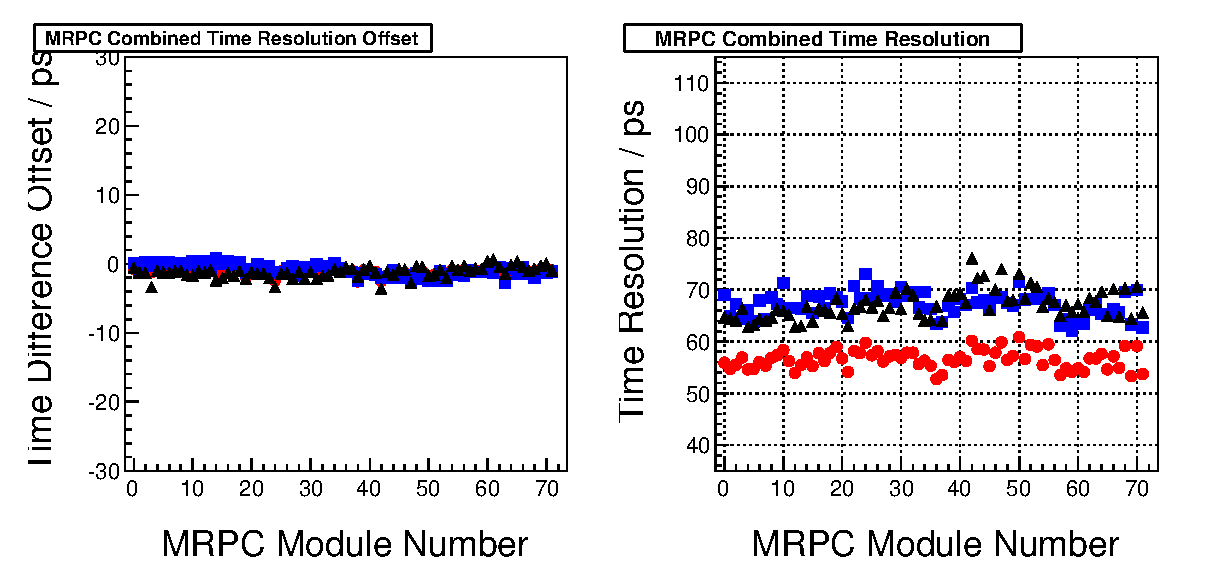
\includegraphics[width=0.9\textwidth]{chap5/calib-res-tofid-combined-160524-30.eps}
\caption{时间分辨随~MRPC~模块的编号的分布}
\label{fig:calib-res-tofid-combined-160524-30}
\end{figure}

\begin{figure}[!h]
\centering
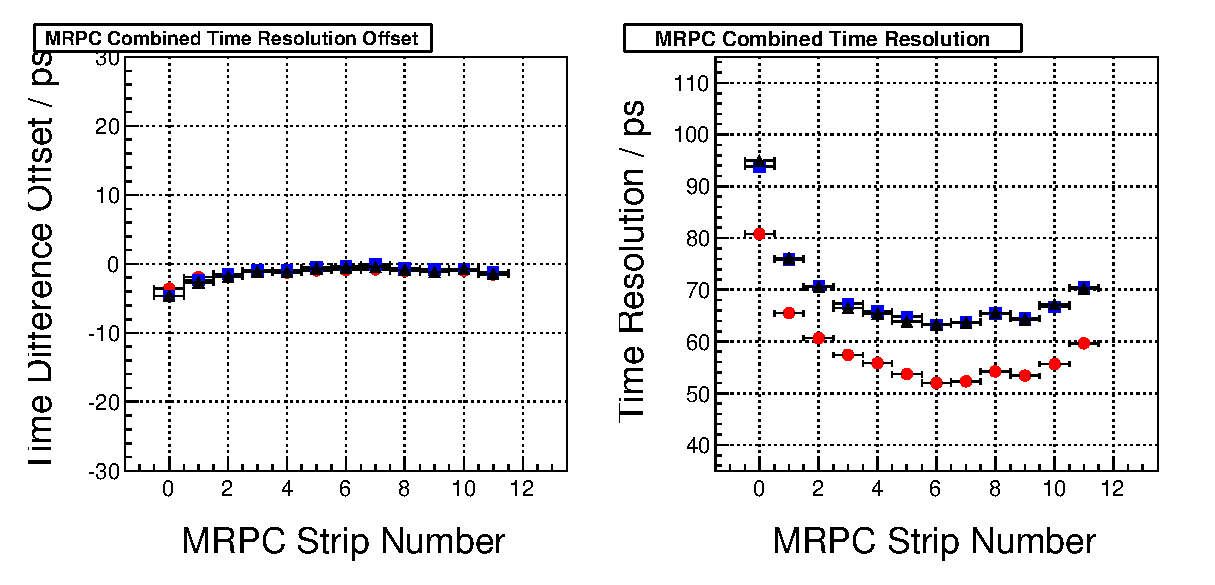
\includegraphics[width=0.9\textwidth]{chap5/calib-res-strip-combined-160524-30.eps}
\caption{时间分辨随~MRPC~读数条的编号的分布}
\label{fig:calib-res-strip-combined-160524-30}
\end{figure}
图~\ref{fig:calib-res-strip-combined-160524-30}~给出的时间刻度后时间分辨随~MRPC~读数条的分布。对于每个读数条的最终时间采用一个高斯拟合,左图是每个读数条的时间采用高斯拟合的中心值分布,右图是高斯拟合得到的方差,也就是模块的时间分辨的分布,其中红色的点表示双端结果,蓝色和黑色的点表示单端的结果。
%这个分布怎么解释????

\begin{figure}[!h]
\centering
\includegraphics[width=1.0\textwidth]{chap5/tofid55-Par2Sca.png}
\caption{模块编号为~55~的双端关于过阈时间刻度项和散点图的关系}
\label{fig:tofid55-Par2Sca}
\end{figure}
图~\ref{fig:tofid55-Par2Sca}~给出了~MRPC~的模块编号为~55~的双端的刻度关于过阈时间项的公式和散点图的关系。可以看出,这个模块~12~个读数条符合的都比较好。说明关于过阈时间的$p_{0}+p_{1}/\sqrt{q}+p_{2}/q$对于整个模块是适用的。

\section{过阈时间和击中位置关联项的研究}
前面研究的都是时间和过阈时间,时间和击中位置之间的关系情况。这一小节主要介绍一下关于过阈时间和击中位置关联项的研究。研究是在本章之前介绍的~7~项公式基础上添加过阈时间和击中位置关联项,然后刻度,然后比较最终得到的时间分辨,时间分辨随模块的编号的分布和时间分辨随读数条的编号的分布等。主要研究了添加~$z/\sqrt{q}+z^{2}/\sqrt{q}$~和~$z/q+z^{2}/q$~的最终结果。
最终得到的分布和不添加这些相关项得到的分布差别不明显。说明,在~7~项公式刻度修正后过阈时间和击中位置之间的关联项的作用很弱。

\begin{table}[h]
    \centering
    \caption{\label{tbl:some-res} 过阈时间和击中位置关联项对时间分辨的影响}
  \footnotesize
    \begin{tabular}{lccc}
        \hline
        公式& 单端left时间分辨(ps)& 单端right时间分辨(ps)& 双端的时间分辨(ps)\\
        \hline
        7项公式& 67.2& 67& 56.6 \\
        7项公式+$z/\sqrt{q}+z^{2}/\sqrt{q}$& 66.7& 66.5& 56.3 \\
        7项公式+$z/q+z^{2}/q$& 66.7& 66.5& 56.3 \\
        \hline
    \end{tabular}
\end{table}

表~\ref{tbl:some-res}~给出了添加关联项后时间分辨的对比情况。可以看出添加的这两种关联项的情况对于最终的时间分辨的影响都是很小的。说明关联比较弱。至于时间随过阈时间,时间随击中位置,以及时间分辨随模块的编号,时间分辨随读数条的编号等的分布变化甚微。

\section{小结}
本章介绍了刻度公式的适用性问题。对~2016~年~5~月~24~日到~5~月~30~日这一周的~Bhabha~数据进行刻度,得到的刻度常数基本稳定,刻度得到的时间分辨随着和模块和读数条的分布基本稳定,确认选用的刻度公式是适用的。之后在此基础上对过阈时间和击中位置的关联项进行了研究,发现它们之间的关联在刻度修正之后比较弱。
%/besfs/groups/cal/tof/guoyx/TofCalib/boss701/TofCalib/final-160524-30/Calib








